To assess the relative importance of the input variables used in the ANN trainings, a feature ranking method was developed. This approach evaluates the trained ANN using a modified test set where each input variable is independently shifted by $\pm 1$ standard deviation. The impact of each shift is quantified by computing the difference between the ANN output for the nominal inputs, and that for the modified inputs. Variables that induce larger changes in the output are considered more influential to the model's decision making.

Certain variables are expected to be more significant based on the kinematic characteristics of the processes involved. For instance, the \wh{} signal process typically exhibits larger \met{} and \metsig{} than the main diboson backgrounds, due to the presence of three neutrinos in the final state. Additionally, the di-lepton mass of the \lzero{} and \lone{} as well as the angular distance between them is expected to be small due to the spin correlation mentioned earlier. The feature ranking method correctly identifies these variables as important to the ANN as seen in Figure~\ref{fig:wh_feature_importance}, demonstrating the reliability of the method. 

\begin{figure}[htp]
  \centering
  \subfloat[\zdom{} feature importance]{
    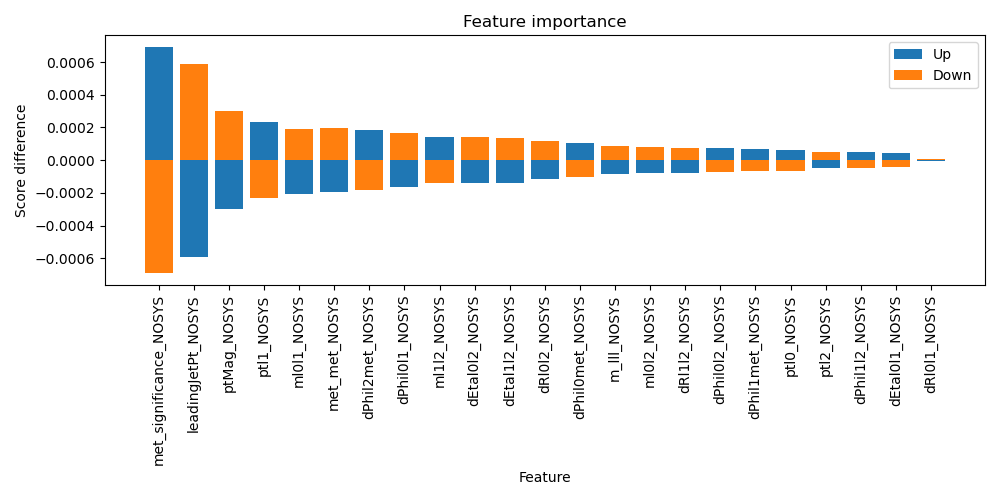
\includegraphics[width=0.9\textwidth]{figures/VH/VH_feature_importance_zdom.png}\label{fig:wh_feature_importance_zdom}
  }
  \hfill
  \subfloat[\zdep{} feature importance]{
    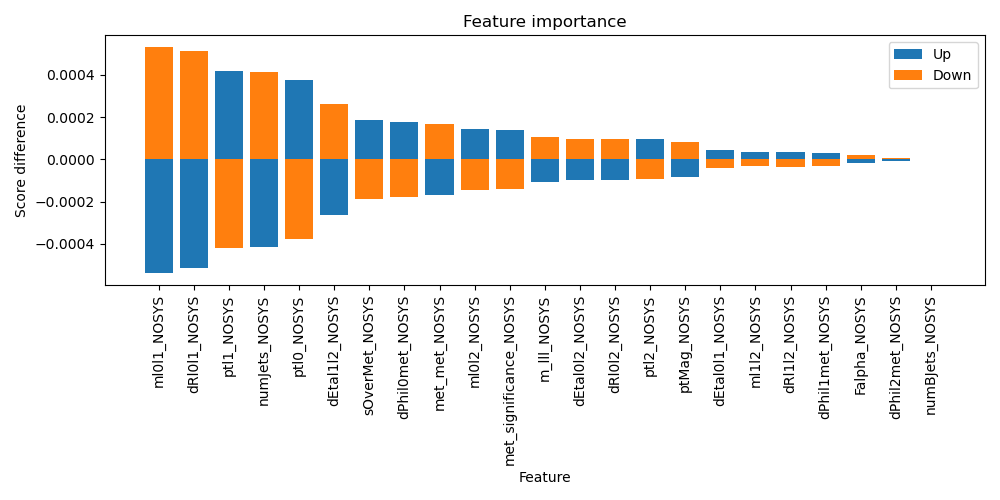
\includegraphics[width=0.9\textwidth]{figures/VH/VH_feature_importance_zdep.png}\label{fig:wh_feature_importance_zdep}
  }
  \caption{Feature importance for the \wh{} analysis. The variables are ranked by their impact on the ANN's output, with the most significant variables towards the left. The \zdom{} channel (a) shows a strong dependence on \met{} and \metsig{}, while the \zdep{} channel (b) has a strong dependence on the di-lepton mass, and the angular distance between the \lzero{} and \lone{} leptons. Additionally, since the training was performed without the $b$-tagged jet veto, this also ranks strongly due to the presence of $b$-jets in $t\bar{t}$ events.}\label{fig:wh_feature_importance}
\end{figure}